\documentclass[a4paper,12pt]{extarticle}
\usepackage[utf8x]{inputenc}
\usepackage[T1,T2A]{fontenc}
\usepackage[russian]{babel}
\usepackage{hyperref}
\usepackage{indentfirst}
\usepackage{listings}
\usepackage{color}
\usepackage{here}
\usepackage{array}
\usepackage{multirow}
\usepackage{graphicx}

\usepackage{caption}
\renewcommand{\lstlistingname}{Программа} % заголовок листингов кода

\bibliographystyle{ugost2008ls}

\usepackage{listings}
\lstset{ %
extendedchars=\true,
keepspaces=true,
language=C,						% choose the language of the code
basicstyle=\footnotesize,		% the size of the fonts that are used for the code
numbers=left,					% where to put the line-numbers
numberstyle=\footnotesize,		% the size of the fonts that are used for the line-numbers
stepnumber=1,					% the step between two line-numbers. If it is 1 each line will be numbered
numbersep=5pt,					% how far the line-numbers are from the code
backgroundcolor=\color{white},	% choose the background color. You must add \usepackage{color}
showspaces=false				% show spaces adding particular underscores
showstringspaces=false,			% underline spaces within strings
showtabs=false,					% show tabs within strings adding particular underscores
frame=single,           		% adds a frame around the code
tabsize=2,						% sets default tabsize to 2 spaces
captionpos=t,					% sets the caption-position to top
breaklines=true,				% sets automatic line breaking
breakatwhitespace=false,		% sets if automatic breaks should only happen at whitespace
escapeinside={\%*}{*)},			% if you want to add a comment within your code
postbreak=\raisebox{0ex}[0ex][0ex]{\ensuremath{\color{red}\hookrightarrow\space}},
texcl=true,
inputpath=listings,                     % директория с листингами
}

\usepackage[left=2cm,right=2cm,
top=2cm,bottom=2cm,bindingoffset=0cm]{geometry}

%% Нумерация картинок по секциям
\usepackage{chngcntr}
\counterwithin{figure}{section}
\counterwithin{table}{section}

%%Точки нумерации заголовков
\usepackage{titlesec}
\titlelabel{\thetitle.\quad}
\usepackage[dotinlabels]{titletoc}

%% Оформления подписи рисунка
\addto\captionsrussian{\renewcommand{\figurename}{Рисунок}}
\captionsetup[figure]{labelsep = period}

%% Подпись таблицы
\DeclareCaptionFormat{hfillstart}{\hfill#1#2#3\par}
\captionsetup[table]{format=hfillstart,labelsep=newline,justification=centering,skip=-10pt,textfont=bf}

%% Путь к каталогу с рисунками
\graphicspath{{fig/}}


\begin{document}	% начало документа

% Титульная страница
\begin{titlepage}	% начало титульной страницы

	\begin{center}		% выравнивание по центру

		\large Санкт-Петербургский политехнический университет Петра Великого\\
		\large Институт компьютерных наук и технологий \\
		\large Кафедра компьютерных систем и программных технологий\\[6cm]
		% название института, затем отступ 6см
		
		\huge Сети и телекоммуникации\\[0.5cm] % название работы, затем отступ 0,5см
		\large Отчет по лабораторной работе\\[0.1cm]
		\large Изучение сокетов и разработка собственных клиент-серверных приложений с помощью протоколов TCP и UDP\\[5cm]

	\end{center}


	\begin{flushright} % выравнивание по правому краю
		\begin{minipage}{0.25\textwidth} % врезка в половину ширины текста
			\begin{flushleft} % выровнять её содержимое по левому краю

				\large\textbf{Работу выполнил:}\\
				\large Сафонов С.В.\\
				\large {Группа:} 43501/1\\
				
				\large \textbf{Преподаватель:}\\
				\large Алексюк А.О.

			\end{flushleft}
		\end{minipage}
	\end{flushright}
	
	\vfill % заполнить всё доступное ниже пространство

	\begin{center}
	\large Санкт-Петербург\\
	\large \the\year % вывести дату
	\end{center} % закончить выравнивание по центру

\thispagestyle{empty} % не нумеровать страницу
\end{titlepage} % конец титульной страницы

\vfill % заполнить всё доступное ниже пространство


% Содержание
% Содержание
\renewcommand\contentsname{\centerline{Содержание}}
\tableofcontents
\newpage




\section{Цель работы}
Целью работы являются изучение основных функций для работы с сокетами со стороны клиента и сервера, а также разработать собственный протокол взаимодействия и создать клиент-серверное приложение, работающего согласно разработанному протоколу.

\section{Программа работы}

\begin{enumerate}
\item Простейшее TCP клиент-серверное приложение
\begin{itemize}
\item Простейший эхо-сервер
\item Многопоточный TCP сервер
\end{itemize}

\item Простейшее UDP клиент-серверное приложение
\begin{itemize}
\item Простейший эхо-сервер
\end{itemize}

\item Разработка TCP приложения по индивидуальному заданию
\begin{itemize}
\item Индивидуальное задание
\item Разработка протокола взаимодействия
\item Написание многопоточного TCP сервера на ОС Linux
\item Написание клиента на ОС Linux
\end{itemize}

\item Разработка UDP приложения по индивидуальному заданию
\begin{itemize}
\item Индивидуальное задание
\item Разработка протокола взаимодействия
\end{itemize}

\item Дополнительное задание
\begin{itemize}
\item Описание задания
\item Выполнение задания
\end{itemize}
\end{enumerate}

\section{Ход выполнения работы}

\subsection{Простейшее TCP клиент-серверное приложение}

\subsubsection{Простейший эхо-сервер}

Для разработки данного приложения необходимо изучить функции работы с сокетами на С.

Для создания сокета применяется функция:
\begin{lstlisting}
int socket(int domain, int type, int protocol);
\end{lstlisting}

Домен определяет пространство адресов, в котором располагается сокет, и множество протоколов, которые используются для передачи данных. Чаще других используются домены Unix и Internet, задаваемые константами AF\_UNIX и AF\_INET соответственно (префикс AF означает "address family" - "семейство адресов"). При задании AF\_UNIX для адресации используется файловая система UNIX. В этом случае сокеты используются для межпроцессного взаимодействия на одном компьютере и не годятся для работы по сети. Константа AF\_INET соответствует Internet-домену. Сокеты, размещенные в этом домене, могут использоваться для работы в любой IP-сети. Существуют и другие домены (AF\_IPX для протоколов Novell, AF\_INET6 для новой модификации протокола IP - IPv6 и т. д.).

Тип сокета определяет способ передачи данных по сети. Чаще других применяются:
\begin{itemize}
\item SOCK\_STREAM. Передача потока данных с предварительной установкой соединения. Обеспечивается надежный канал передачи данных, при котором фрагменты отправленного блока не теряются, не переупорядочиваются и не дублируются. Поскольку этот тип сокетов является самым распространенным, до конца раздела мы будем говорить только о нём. Остальным типам будут посвящены отдельные разделы.
\item SOCK\_DGRAM. Передача данных в виде отдельных сообщений (датаграмм). Предварительная установка соединения не требуется. Обмен данными происходит быстрее, но является ненадежным: сообщения могут теряться в пути, дублироваться и переупорядочиваться. Допускается передача сообщения нескольким получателям (multicasting) и широковещательная передача (broadcasting).
\item SOCK\_RAW. Этот тип присваивается низкоуровневым (т. н. "сырым") сокетам. Их отличие от обычных сокетов состоит в том, что с их помощью программа может взять на себя формирование некоторых заголовков, добавляемых к сообщению.
\end{itemize}
Для реализации SOCK\_STREAM используется протокол TCP, для реализации SOCK\_DGRAM - протокол UDP,

Прежде чем передавать данные через сокет, его необходимо связать с адресом в выбранном домене  с помощью функции:
\begin{lstlisting}
int bind(int sockfd, struct sockaddr *addr, int addrlen);
\end{lstlisting}
В качестве первого параметра передается дескриптор сокета, который мы хотим привязать к заданному адресу. Второй параметр, addr, содержит указатель на структуру с адресом, а третий - длину этой структуры.
Структура sockaddr иммет следующий вид:
\begin{lstlisting}
struct sockaddr {
    unsigned short    sa_family;    // Семейство адресов, AF\_xxx
    char              sa_data[14];  // 14 байтов для хранения адреса
};
\end{lstlisting}

Работать с этой структурой напрямую не очень удобно, поэтому будем использовать вместо sockaddr одну из альтернативных структур вида sockaddr\_XX (XX - суффикс, обозначающий домен: "un" - Unix, "in" - Internet и т. д.).При передаче в функцию bind указатель на эту структуру приводится к указателю на sockaddr. Рассмотрим для примера структуру sockaddr\_in:
\begin{lstlisting}
struct sockaddr_in {
    short int          sin_family;  // Семейство адресов
    unsigned short int sin_port;    // Номер порта
    struct in_addr     sin_addr;    // IP-адрес
    unsigned char      sin_zero[8]; // "Дополнение" до размера структуры sockaddr
};
\end{lstlisting}

На следующем шаге создается очередь запросов на соединение. При этом сокет переводится в режим ожидания запросов со стороны клиентов:
\begin{lstlisting}
int listen(int sockfd, int backlog);
\end{lstlisting}
Первый параметр - дескриптор сокета, а второй задает размер очереди запросов.

Когда сервер готов обслужить очередной запрос, он использует функцию accept:
\begin{lstlisting}
int accept(int sockfd, void *addr, int *addrlen);
\end{lstlisting}
Функция accept создает для общения с клиентом новый сокет и возвращает его дескриптор. Параметр sockfd задает слушающий сокет. После вызова он остается в слушающем состоянии и может принимать другие соединения. В структуру, на которую ссылается addr, записывается адрес сокета клиента, который установил соединение с сервером.

После того как соединение установлено, можно начинать обмен данными. Для этого используются функции send и recv в ОС Windows и read и write в ОС Linux:
\begin{lstlisting}
int send(int sockfd, const void *msg, int len, int flags);
int recv(int sockfd, const void *msg, int len, int flags);
\end{lstlisting}
Здесь sockfd - это дескриптор сокета, через который мы отправляем данные, msg - указатель на буфер с данными для send и буфер для приема данных для recv, len - длина буфера в байтах(сколько будет передано/считано), а flags - набор битовых флагов, управляющих работой функции.
\begin{lstlisting}
int write(int sockfd, const void *msg, int len);
int read(int sockfd, const void *msg, int len);
\end{lstlisting}
Функции для ОС Linux отличаются лишь отсутствием флагов.

Для закрытия сокета используются функции shutdown и close:
\begin{lstlisting}
int shutdown(int sockfd, int how);
int close(int fd);
\end{lstlisting}
С помощью shutdown можно закрыть сокет для передачи в каком-то направлении с помощью параметра how: 0 - запретить чтение, 1 - запретить запись, 2 - запретить и то и то.
Close() освобождает связанные с сокетом системные ресурсы.

С стороны клиента также установить соединение с сокетом, который будет открыт командой accept() сервера. Для этого используется функция connect:
\begin{lstlisting}
int connect(int sockfd, struct sockaddr *serv\_addr, int addrlen);
\end{lstlisting}
Здесь sockfd - сокет, который будет использоваться для обмена данными с сервером, serv\_addr содержит указатель на структуру с адресом сервера, а addrlen - длину этой структуры.

Порядок вызовов функций для работы с сокетами на стороне эхо-сервера:
\begin{itemize}
\item socket() - создает сокет
\item bind() - привязка созданного сокета к заданным IP-адресам и портам
\item listen() - переводит сокет в состояние прослушивания
\item accept() - принимает поступающие запросы на подключение и возвращает сокет для нового соединения
\item recv() - чтение данных от клиента из сокета, возвращенного на предыдущем шаге
\item send() - отправка только что принятых данных клиенту
\item shutdown() - разрыв соединения с клиентом
\item close() - для закрытия клиентского и слушающего сокетов
\end{itemize}

Порядок вызовов функций для работы с сокетами на стороне клиента:
\begin{itemize}
\item socket() - создает сокет
\item connect() - установка соединения для сокета, который будет связан с серверным сокетом, порожденным вызовом accept()
\item send() - отправка данных серверу
\item recv() - чтение тех же данных от сервера
\item shutdown() - разрыв соединения с клиентом
\item close() - для закрытия клиентского и слушающего сокетов
\end{itemize}

\subsubsection{Многопоточный TCP сервер}
Для организации работы сервера с множеством клиентов необходимо сделать следующее:
\begin{itemize}
\item Вынести общение с клиентом (send и recv) в отдельную функцию для того, чтобы была возможность вызывать ее в новом потоке.
\item Организовать работу функций listen() и accept() в цикле.
listen() должен работать с первым слушающий сокетом, а accept каждый раз будет создавать новый сокет для общения с клиентом.
\item Открывать новый поток, вызывая функцию общения с клиентом.
В функцию общения с клиентом необходимо передавать новый сокет, дескриптор которого возвращает accept.
\end{itemize}
Написанная функция общения с клиентом:
\begin{lstlisting}
void* connection_hadler (void* temp);
\end{lstlisting}
Функция принимает в качестве аргумента ссылку на дескриптор сокета. Возвращаемый результат void* и тип аргумента void * необходимы для вызова функции в новом потоке.
Преобразование аргумента в целочисленный дескриптор происходит следующим образом:
\begin{lstlisting}
int sock = *((int *) temp);
\end{lstlisting}

Вызов функций listen() и accept() выполнен в цикле:
\begin{lstlisting}
while(1){
        listen(sockfd, 5);
        newsockfd = accept(sockfd, (struct sockaddr *) &cli_addr, &(sizeof(cli_addr)));
	.....
}
\end{lstlisting}

После открытия нового сокета создается поток. В качестве аргументов ему передается функция работы с клиентом как стартовая функция работы потока, а также дескриптор сокета, чтобы его получила функция общения с клиентом. Создание такого потока на примере сервера на ОС Linux:
\begin{lstlisting}
while(1){
	....
        pthread_t tid;
        pthread_create(&tid, NULL,  connection_hadler, &newsockfd);
        pthread_detach(tid);
}
\end{lstlisting}

\subsection{Простейший UDP клиент-сервер}
Для организации обмена через UDP и обмена с помощью датаграмм необходимо внести следующие изменения в функцию создания сокета, изменить функции чтения и записи, а также изменить порядок вызовов функций.

При создании сокетов как на стороне сервера, так и на стороне клиента, необходимо вторым аргументом (тип данных) передать константу SOCK\_DGRAM, для организации передачи датаграммами без подтверждения соединения.

Также при передаче через UDP изменятся функции чтения и передачи сообщений:
\begin{lstlisting}
ssize_t recvfrom(int sockfd, void *buf, size_t len, int flags, struct sockaddr *src_addr, socklen_t *addrlen);
ssize_t sendto(int sockfd, const void *buf, size_t len, int flags, const struct sockaddr *dest_addr, socklen_t addrlen);
\end{lstlisting}
В качестве аргументов передаются дескриптор сокета, буфер для чтения/записи, флаги. структура с информацией о передающей/принимабщей стороне, длина этой структуры.
Возвращаемое значение - число реально принятых/переданных символов.

Изменится и состав вызова функций для работы с сокетами на клиенте и сервере. 
Порядок действий сервера:
\begin{itemize}
\item socket() - создает сокет
\item bind() - привязка созданного сокета к заданным IP-адресам и портам
\item recfrom() - чтение данных от клиента из сокета, возвращенного на предыдущем шаге
\item sendto() - отправка только что принятых данных клиенту
\item shutdown() - разрыв соединения с клиентом
\item close() - для закрытия клиентского и слушающего сокетов
\end{itemize}
Для организации обмена по UDP не происходит прослушивание сокетом на подключение и подтверждения соединения с созданием нового сокета.

Порядок действий клиента:
\begin{itemize}
\item socket() - создает сокет
\item connect() - установка соединения для сокета, который будет связан с серверным сокетом, порожденным вызовом accept()
\item sendto() - отправка данных серверу
\item recvfrom() - чтение тех же данных от сервера
\item shutdown() - разрыв соединения с клиентом
\item close() - для закрытия клиентского и слушающего сокетов
\end{itemize}
Действия клиента не меняются, однако возможно не использовать подтверждение соединения с помощью connect()

\subsection{Разработка TCP приложения по индивидуальному заданию}
\subsubsection{Индивидуальное задание}
В качестве индивидуального задания была выбрана система распределенных математических расчетов. Сервер и клиент реализованы на ОС Linux.

Серверное приложение реализует следующие функции:
\begin{itemize}
	\item Прослушивание определенного порта
	\item Обработка запросов на подключение по этому порту от клиентов
	\item Поддержка одновременной работы нескольких клиентов с использованием механизма нитей и средств синхронизации доступа к разделяемым между нитями ресурсам
	\item Принудительное отключение конкретного клиента
	\item Хранение рассчитанных клиентами простых чисел, а также текущей
	нижней границы диапазона для нового запроса на расчет
	\item Выдача клиентам максимального рассчитанного простого числа
	\item Выдача клиентам последних N рассчитанных простых чисел
	\item Выдача клиентам необходимого диапазона расчета чисел
	\item * Сохранение состояния при выключении сервера
\end{itemize}

Клиентское приложение реализует следующие функции:

\begin{itemize}
	\item Возможность параллельной работы нескольких клиентов с одного
	или нескольких IP-адресов
	\item Установление соединения с сервером (возможно, с регистрацией на
	сервере)
	\item Разрыв соединения
	\item Обработка ситуации отключения сервером
	\item Получение от сервера и вывод максимально рассчитанного простого
	числа
	\item Получение от сервера и вывод последних N рассчитанных простых
	чисел
	\item Получение от сервера диапазона расчета простых чисел (нижнюю
	грань выдает сервер, количество проверяемых чисел - клиент)
	\item Расчет простых чисел в требуемом диапазоне (имеет смысл проверять остатки от деления на все нечетные числа в пределах
	sqrt(Nmax)+1)
	\item Передача серверу набора рассчитанных простых чисел
\end{itemize}

Сначала необходимо разработать собственный протокол взаимодействия клиента и сервера. Далее необходимо написать клиент-серверное приложение , работающее согласно разработанному протоколу и реализующее заданную функциональность.
\subsubsection{Разработка протокола взаимодействия}

Протокол взаимодействия осуществяется через общение клиента с сервером, заключающееся в отправке клиентом запроса с командой серверу, обработке сервером полученного запроса и отправке клиенту ответа с необходимыми данными.

После считывания команды из консоли, клиент запускает процедуру разделения полученной строки для получения аргумента и определения, какая команда была введена. Если введенная команда не совпадает ни с одной из 10 возможных, то выводится сообщение "Unknown type of request", и приложение ждет ввода новой команды. Если было обнаружено совпадение с одной из возможных команд, то вызывается функция общения с сервером. Далее представлено взаимодействие клиента и сервера друг с другом при вводе различных команд.

\begin{itemize}
\item Команда регистрации пользователя в базе сервера (REG <login>)
\end{itemize}

Клиент посылает посылку серверу с именем пользователя, которого нужно занести в папку пользователей. После этого сервер проверяет запрос на ошибки и на существование данного имени пользователя в базе. При наличии имени клиенту высылается ответ с сообщением, иначе сервер создаёт бинарный файл с именем соответствующего пользователя и файл сессии для работы с ним. Клиент получает результат запроса и логинится под данным именем для дальнейшей работы (большинство запросов не выполняются для пользователей со статусом 'new-user').

\begin{itemize}
\item Команда авторизации на сервере по имени пользователя (LOGIN <login>)
\end{itemize}

Алгоритм работы аналогичен работе запроса о регистрации пользователя, за исключением того, что сервер проверяет высылает уведомление клиенту о несуществующем пользователей в ходе проверки своей базы.

\begin{itemize}
\item Команда удаления текущего пользователя из базы и его отключение сервером (DEL)

\end{itemize}

После получения запроса сервер проверяет наличия клиента, который послал запрос, в текущей сессии. В случае отсутствия высылается уведомление, иначе сервер удаляет бинарный файл с именем клиента из базы. После получения ответа клиент получает статус 'not-logged' и также, как и 'new-user', должен предварительно зарегистрироваться или авторизоваться для дальнейшей работы.

\begin{itemize}
\item Команда передачи максимального вычисленного простого числа (MAXPRIME)
\end{itemize}

Сервер просматривает все вычисленные простые числа с целью найти максимальное (реализуется простой поиск максимума в массиве). После этого найденный максимум высылается клиенту и выводится в консоль.

\begin{itemize}
	\item Команда передачи последних вычисленных N простых чисел (PRIMES <N>)
\end{itemize}

Сервер просматривает все вычисленные простые числа с целью найти максимальное (реализуется простой поиск максимума в массиве) и находит его индекс. После этого в цикле он производит выборку последних N простых чисел, начиная с максимума в обратную сторону. Полученный массив чисел высылается клиенту и выводится в консоль.

\begin{itemize}
	\item Команда передачи значения диапазона для вычислений (RANGE)
\end{itemize}

Сервер высылает клиенту значение диапазона, на котором будет выполняться вычисление простых чисел.

\begin{itemize}
	\item Команда выполнения расчёта простых чисел клиентом (CALC)
\end{itemize}

В начале сервер высылает клиенту сообщение с рассчитанным диапазоном расчёта простых чисел, а также текущий диапазон и диапазон для расчёта. После получения посылки клиентом реализуется алгоритм вычисления и записи полученных значений в символьный массив. Полученный массив пересылается на сервер, где значения записываются в текущую базу значений. В конце производится запись всей текущей базы в файл, отвечающий за состояние сервера, из которого сервер вытаскивает данные при начале нового сеанса.

Для оптимизации работы и исключения появления ошибок сегментации было решено хранить в базе сервера 50 последних выполненных простых чисел.

\begin{itemize}
	\item Команда очистки данных с сервера (CLEAR)
\end{itemize}

Сервер обнуляет массив хранения простых чисел и текущий диапазон расчёта в текущей базе значений.

\begin{itemize}
	\item Команда разрыва соединения клиентом (QUIT)
\end{itemize}

На стороне сервера удаляется сессия работы с текущим клиентом и закрывается поток и сокет. Клиент завершает свою работу.

\begin{itemize}
	\item Команда вызова справки (HELP)
\end{itemize}

В консоль выводится описания всех возможных команд клиент-серверного приложения.

\subsubsection{Написание многопоточного TCP сервера на ОС Linux}
Основная логика создания сокетов, привязка их к адресам, выделения новых потоков для общения с клиентами осталась такой же, как и в простейшем многопоточном эхо-сервере.

Для отслеживания запросов и ответов, а также для определения команды были созданы соответствующие структуры: 

\begin{itemize}
	\item Структура команд хранит в себе один из десяти типов команды и аргумент (если он присутствует).
	
	\begin{lstlisting}
	struct command {
		char* type;
		char* arg1;
	};
	\end{lstlisting}
	
	\item Структура запроса содержит поле типа структуры команд и токен сессии, в которой работает текущий клиент.
	
	\begin{lstlisting}
	struct request {
		struct command comm;
		char* token;
	};
	\end{lstlisting}
	
	\item Структура реакции на запрос хранит тип возвращаемого ответа (ошибка, нормальная работа, удаление и текущий токен при авторизации) и содержимое ответа.
	
	\begin{lstlisting}
	struct response {
		char* type;
		char* payload;
	};
	\end{lstlisting}
\end{itemize}

Для отслеживания клиентов при каждом появлением нового пользователя создаётся и присваивает новый поток, в котором выполняется обработка запросов от него до тех пор, пока клиент сам не захочет закончить сеанс.

Процедура приёма запроса заключается в принятии длины ответа и бинарного массива, в котором содержатся данные ответа. Большую часть тела процедуры занимает преобразование бинарного массива в соответствующую структуру.

\begin{lstlisting}
int get_request(int sockfd, struct request* req)
{
	int readRes; // Result of reading
	char* buf; // Buffer for reading
	int message_length; // Length of message without first sizeof(int) bytes

	int arg_length;
	int buf_pointer = 0;

	// Get length of request
	buf = (char*)malloc(sizeof(int));
	readRes = read_socket(sockfd, buf, sizeof(int));

	if (readRes != WORKING_SOCKET) {
		return readRes;
	}

	message_length = *(int*)buf;
	if (message_length <= 0 || message_length > 1024) {
		return REQUEST_LENGTH_ERROR;
	}

	// Clear memory
	free(buf);

	// Read byte array of request
	buf = (char*)malloc(message_length * sizeof(char));

	readRes = read_socket(sockfd, buf, message_length);

	if (readRes != WORKING_SOCKET) {
		return readRes;
	}

	// Now convert byte array to request struct
	// Get length of type
	bcopy(&buf[buf_pointer], &arg_length, sizeof(int));
	buf_pointer += sizeof(int);

	// Get type of request
	req->comm.type = (char*)malloc(arg_length * sizeof(char) + 1);
	bzero(req->comm.type, arg_length * sizeof(char) + 1);
	bcopy(&buf[buf_pointer], req->comm.type, arg_length * sizeof(char));
	buf_pointer += arg_length * sizeof(char);

	// Get length of arg1
	bcopy(&buf[buf_pointer], &arg_length, sizeof(int));
	buf_pointer += sizeof(int);

	// Get arg1
	if (arg_length > 0) {
		req->comm.arg1 = (char*)malloc(arg_length * sizeof(char) + 1);
		bzero(req->comm.arg1, arg_length * sizeof(char) + 1);
		bcopy(&buf[buf_pointer], req->comm.arg1, arg_length * sizeof(char));
		buf_pointer += arg_length;
	} else {
		req->comm.arg1 = 0;
	}

	// Get token
	if (message_length - buf_pointer == 0) {
		req->token = 0;
	} else {
		arg_length = message_length - buf_pointer;
		req->token = (char*)malloc(arg_length * sizeof(char) + 1);
		bzero(req->token, arg_length * sizeof(char) + 1);
		bcopy(&buf[buf_pointer], req->token, arg_length * sizeof(char));
	}

	// Clear memory
	free(buf);

	return WORKING_SOCKET;
}
\end{lstlisting}

После определения типа запроса выполняется одна из 10 операций, каждая из которых заканчивается отправкой результата работы клиента. За отправку отвечает процедура response\_request. Общая длина ответа равна совокупности длин типа ответа и его содержимого.

\begin{lstlisting}
int response_request(int sockfd, char* type, char* payload)
{
	int type_length; // Length of response type
	int payload_length; // Length of payload type
	int length; // Total length of response
	char* buf; // Buffer for response

	int res;
	int buf_pointer = 0;

	// Set type length
	type_length = strlen(type);

	// Set payload length
	payload_length = strlen(payload);

	// Count total length of response
	length = sizeof(int) * 2 + (type_length + payload_length) * sizeof(char);

	// Send length to client
	res = send(sockfd, &length, sizeof(int), NULL);
	if (res < 0) {
		return WRITING_ERROR;
	}

	// Allocate memory
	buf = (char*)malloc(length);
	bzero(buf, length);

	// Set response type length
	bcopy(&type_length, &buf[buf_pointer], sizeof(int));
	buf_pointer += sizeof(int);

	// Set response type
	bcopy(type, &buf[buf_pointer], type_length * sizeof(char));
	buf_pointer += type_length * sizeof(char);

	// Set response payload length
	bcopy(&payload_length, &buf[buf_pointer], sizeof(int));
	buf_pointer += sizeof(int);

	// Set response payload
	bcopy(payload, &buf[buf_pointer], payload_length * sizeof(char));
	buf_pointer += payload_length * sizeof(char);

	// Send response to client
	res = send(sockfd, buf, length, NULL);
	free(buf);

	if (res < 0) {
		return WRITING_ERROR;
	}

	return WORKING_SOCKET;
}
\end{lstlisting}

Для описания реакций на всевозможные ошибки, возникающие в ходе работы приложения, была создана отдельная процедура-обработчик ошибок. В связи с этим клиент может точно отобразить тип ошибки в рабочей консоли.

\begin{lstlisting}
int handle_errors(int sockfd, int error)
{
	switch (error) {
		case OK:
			return 0;
		case USER_ALREADY_EXISTS:
			send_response(sockfd, RESPONSE_ERROR, "User already exists");
			return 1;
		case USER_NOT_FOUND:
			send_response(sockfd, RESPONSE_ERROR, "User not found");
			return 1;
		case OPEN_FILE_ERROR:
			send_response(sockfd, RESPONSE_ERROR, "Can't open file");
			return 1;
		case READ_FILE_ERROR:
			send_response(sockfd, RESPONSE_ERROR, "Can't read from file");
			return 1;
		case WRITE_FILE_ERROR:
			send_response(sockfd, RESPONSE_ERROR, "Can't write to file");
			return 1;
		case CLOSE_FILE_ERROR:
			send_response(sockfd, RESPONSE_ERROR, "Can't close file");
			return 1;
		case BOUND_IS_NOT_MULTIPLE:
			send_response(sockfd, RESPONSE_ERROR, "Bound must be multiple to range or equal 0");
			return 1;
		case RANGE_IS_ALREADY_USED:
			send_response(sockfd, RESPONSE_ERROR, "Bound is already used");
			return 1;
		case NEGATIVE_BOUND:
			send_response(sockfd, RESPONSE_ERROR, "Bound can't be negative");
			return 1;
		case INCORRECT_BOUNDS:
			send_response(sockfd, RESPONSE_ERROR, "Upper bound must be larger than lower bound");
			return 1;
		case INCORRECT_COUNT:
			send_response(sockfd, RESPONSE_ERROR, "Count must be larger than 0 and less than array of primes size");
			return 1;
		case OTHER_ERROR:
			send_response(sockfd, RESPONSE_ERROR, "Internal error");
			return 1;
		case READING_ERROR:
			close_socket(sockfd, "ERROR while reading from socket");
			pthread_exit(0);
		case WRITING_ERROR:
			close_socket(sockfd, "ERROR while writing to socket");
			pthread_exit(0);
		case READING_IS_NOT_FINISHED:
			close_socket(sockfd, "Client closed connection");
			pthread_exit(0);
		case REQUEST_LENGTH_ERROR:
			close_socket(sockfd, "ERROR in request length");
			pthread_exit(0);
		default:break;
	}
	return 0;
}
\end{lstlisting}

В дополнение ко всему, отдельными процедурами были реализованы проверка корректности полученного вместе с запросом аргумента, который зависит от типа команды и крайних значений, и проверка достоверности токена сессии, в которой работает текущий клиент.

\begin{lstlisting}
// Function for checking arguments
int check_arguments(int sockfd, struct request req)
{
	// Check if arguments are NULL

	if (req.comm.arg1 == NULL) {
		send_response(sockfd, RESPONSE_ERROR, "Illegal argument");
		return 1;
	}
	return 0;
}

// Function for checking token
int check_token(int sockfd, struct request req)
{
	// Check if token is NULL
	if (req.token == NULL) {
		send_response(sockfd, RESPONSE_ERROR, "You are not logged");
		return 1;
	}
	return 0;
}
\end{lstlisting}

\subsubsection{Написание клиента на ОС Linux}

После подключения клиента к серверу, второй начинает ожидать присланной ему команды от клиента. Соответственно клиент имеет 10 команд, которые считываются из консоли, куда их вводит пользователь. Пользователь вводит команду следующего вида:

\begin{lstlisting}
<command> <argument>
\end{lstlisting}

При соединении клиента с сервером в начале определяется длина запроса с целью проверки целостности посылки, а затем сам запрос, после чего вызывается функцию разделения. 

Функция parse\_request разделяет принятое сообщение на команду и аргумент, проверяет команду и вызывает функцию обработки команды:

\begin{lstlisting}
int parse_request(char* str, struct request* req)
{
	char* str_token; // First found token in the string str

	// Get type of request
	str_token = strtok(str, " \n");
	if (str_token == NULL)
		return INVALID_REQUEST;
	req->comm.type = str_token;

	// Get arg1
	str_token = strtok(NULL, " \n");
	if (str_token == NULL) {
		req->comm.arg1 = 0;
		return WORKING_SOCKET;
	}
	req->comm.arg1 = str_token;

	return WORKING_SOCKET;
}
\end{lstlisting}

После записи токена сессии в структуру запроса, выполняется операция отправки запроса серверу, по структуре схожая с процедурой отправки ответа клиенту. Общая длина сообщения определяется из совокупных длин типа запроса, аргумента (если есть) и токена сессии.

\begin{lstlisting}
	// Count total length of request
	length = sizeof(int) * 3 + (type_length + arg1_length + token_length) * sizeof(char);
\end{lstlisting}

Процедура приёма ответа аналогична по струтуре процедуре приёма запроса сервером.

Последние операции, которые выполняет клиент - это вызов обработчиков, зависящих от типа полученного ответа от сервера или выбора клиентом команды QUIT.

\begin{lstlisting}
	// Handle response
	if (strcmp(resp.type, RESPONSE_TOKEN) == 0) {
	strcpy(token, resp.payload);
	strcpy(login, req.comm.arg1);
	printf("You are logged as %s\n", login);
	}
	
	if (strcmp(resp.type, RESPONSE_DELETED) == 0) {
		bzero(token, 50);
		printf("Session is over\n");
		strcpy(login, "not-logged");
	}
	
	if (strcmp(resp.type, RESPONSE_OK) == 0) {
		printf("%s\n", resp.payload);
	}
	
	if (strcmp(resp.type, RESPONSE_ERROR) == 0) {
		printf("ERROR: %s\n", resp.payload);
	}
	
	if (strcmp(req.comm.type, "QUIT") == 0) {
		break;
	}
\end{lstlisting}

\subsection{Разработка UDP приложения по индивидуальному заданию}
\subsubsection{Индивидуальное задание}
Функциональные требования к приложению остались теми же, как и у TCP приложения. Отличие от TCP приложения: необходимо добавить контроль номера принятых и посланных пакетов, чтобы определить случаи потери или перемешивания пакетов.
\subsubsection{Разработка протокола взаимодействия}
Основные особенности протокола в формате и длине пакетов остались без изменений, однако для структур запроса и ответа введено поле, отвечающее за номер сообщения.

UDP сервер был написан на основе TCP сервера, описанного выше. Отличия от TCP сервера:
\begin{enumerate}
\item Для первого запроса записывается номер, равный 1 и который увеличивается при каждом новом запросе 
\item После обработки запроса от клиента сервер записывает номер ответа, равный номеру запроса
\item Клиент получает ответ от сервера и первоначально сравнивает номера запроса и ответа
\item В случае несовпадения происходит обработка ошибки о потере и перемешивании пакетов
\end{enumerate}

Для отправки номера сообщения в метод send\_request добавлен вызов функции sendto.
\begin{lstlisting}
res = sendto(sockfd, &index, sizeof(int), 0, (struct sockaddr *) serv_addr, sizeof(*serv_addr));
if (res == -1) {
	close_socket(sockfd, "ERROR write length to socket");
	return -1;
}

req->index = index;
}
\end{lstlisting}

В функции приёма ответа от сервера добавлена проверка на соответствие номеров запроса и ответа.

\begin{lstlisting}
buf = (char*)malloc(sizeof(int));
res = read_socket(sockfd, buf, sizeof(int), serv_addr);
// Throw errors
if (res != WORKING_SOCKET) {
	return res;
}

num = *(int*)buf;
if (num != req->index) {
	return LOST_OR_WRONG_PACKET;
}
resp->index = num;
\end{lstlisting}

\subsection{Дополнительное задание}
Попробовать проанализировать код с помощью статического и динамического анализатора. Когда закончите индивидуальные задания, проверьте исходный код своих программ с помощью clang-tidy и cppcheck. При запуске утилит включайте все доступные проверки. После этого проверьте с помощью valgrind свои программы на предмет утечек памяти и неправильного использования многопоточности. Опишите все найденные ошибке в отчете, а также укажите, как их можно исправить.

\subsubsection{Выполнение задания}

\begin{itemize}
	\item Статические анализаторы кода

Статический анализ кода - это процесс выявления ошибок и недочетов в исходном коде программ. Он заключается в совместном внимательном чтении исходного кода и высказывании рекомендаций по его улучшению. В процессе чтения кода выявляются ошибки или участки кода, которые могут стать ошибочными в будущем. Главное преимущество статического анализ состоит в возможности существенной снижении стоимости устранения дефектов в программе. 

Задачи, решаемые программами статического анализа кода можно разделить на 3 категории:

\begin{enumerate}
	\item Выявление ошибок в программах
	\item Рекомендации по оформлению кода
	\item Подсчет метрик
\end{enumerate}

Преимущества статических анализаторов кода:

\begin{itemize}
	\item Полное покрытие кода.Статические анализаторы проверяют даже те фрагменты кода, которые получают управление крайне редко. Такие участки кода, как правило, не удается протестировать другими методами.
	\item Статический анализ не зависит от используемого компилятора и среды, в которой будет выполняться скомпилированная программа. Это позволяет находить скрытые ошибки, которые могут проявить себя только через несколько лет.
	\item Можно легко и быстро обнаруживать опечатки и последствия использования Copy-Paste. Как правило, нахождение этих ошибок другими способами является кране неэффективной тратой времени и усилий. 
\end{itemize}

В качестве статических анализаторов были выбраны утилиты clang-tidy и cppcheck в связи с тем, что приложение было написано на языке C. Проверка была проведена для варианта индивидуального задания для протокола TCP.

Проверка сервера с помощью clang-tidy:

\begin{lstlisting}
	/home/mrsandman/CLionProjects/server_linux/main.c:47:27: warning: statement should be inside braces [google-readability-braces-around-statements]
	if (strlen(buff) != 0) retrieve_data(&data, buff);
	^
	{
	/home/mrsandman/CLionProjects/server_linux/main.c:48:9: warning: statement should be inside braces [hicpp-braces-around-statements]
	else clear_data(&data);
	^
	{
	/home/mrsandman/CLionProjects/server_linux/main.c:58:25: warning: prefer accept4() to accept() because accept4() allows SOCK_CLOEXEC [android-cloexec-accept]
	while ((newsockfd = accept(sockfd, (struct sockaddr*)&cli_addr, &clilen))) {
	^~~~~~~~~~~~~~~~~~~~~~~~~~~~~~~~~~~~~~~~~~~~~~~~~~~~~
	accept4(sockfd, (struct sockaddr*)&cli_addr, &clilen, SOCK_CLOEXEC)
	/home/mrsandman/CLionProjects/server_linux/main.c:92:40: warning: statement should be inside braces [google-readability-braces-around-statements]
	if (handle_errors(sockfd, res))
	^
	{
	/home/mrsandman/CLionProjects/server_linux/main.c:126:38: warning: statement should be inside braces [readability-braces-around-statements]
	if (check_arguments(sockfd, req))
	^
	{
	/home/mrsandman/CLionProjects/server_linux/main.c:145:36: warning: statement should be inside braces [google-readability-braces-around-statements]
	if (handle_errors(sockfd, res))
	^
	{
	/home/mrsandman/CLionProjects/server_linux/main.c:151:36: warning: statement should be inside braces [google-readability-braces-around-statements]
	if (handle_errors(sockfd, res))
	^
	{
	/home/mrsandman/CLionProjects/server_linux/main.c:162:38: warning: statement should be inside braces [google-readability-braces-around-statements]
	if (check_arguments(sockfd, req))
	^
	{
	/home/mrsandman/CLionProjects/server_linux/main.c:174:36: warning: statement should be inside braces [readability-braces-around-statements]
	if (handle_errors(sockfd, res))
	^
	{
	/home/mrsandman/CLionProjects/server_linux/main.c:180:36: warning: statement should be inside braces [hicpp-braces-around-statements]
	if (handle_errors(sockfd, res))
	^
	{
	/home/mrsandman/CLionProjects/server_linux/main.c:190:34: warning: statement should be inside braces [google-readability-braces-around-statements]
	if (check_token(sockfd, req))
	^
	{
	/home/mrsandman/CLionProjects/server_linux/main.c:196:36: warning: statement should be inside braces [google-readability-braces-around-statements]
	if (handle_errors(sockfd, res))
	^
	{
	/home/mrsandman/CLionProjects/server_linux/main.c:199:36: warning: statement should be inside braces [google-readability-braces-around-statements]
	if (handle_errors(sockfd, res))
	^
	{
	/home/mrsandman/CLionProjects/server_linux/main.c:204:36: warning: statement should be inside braces [google-readability-braces-around-statements]
	if (handle_errors(sockfd, res))
	^
	{
	/home/mrsandman/CLionProjects/server_linux/main.c:214:34: warning: statement should be inside braces [google-readability-braces-around-statements]
	if (check_token(sockfd, req))
	^
	{
	/home/mrsandman/CLionProjects/server_linux/main.c:231:34: warning: statement should be inside braces [google-readability-braces-around-statements]
	if (check_token(sockfd, req))
	^
	{
	/home/mrsandman/CLionProjects/server_linux/main.c:235:38: warning: statement should be inside braces [google-readability-braces-around-statements]
	if (check_arguments(sockfd, req))
	^
	{
	/home/mrsandman/CLionProjects/server_linux/main.c:243:36: warning: statement should be inside braces [google-readability-braces-around-statements]
	if (handle_errors(sockfd, res))
	^
	{
	/home/mrsandman/CLionProjects/server_linux/main.c:253:34: warning: statement should be inside braces [google-readability-braces-around-statements]
	if (check_token(sockfd, req))
	^
	{
	/home/mrsandman/CLionProjects/server_linux/main.c:268:34: warning: statement should be inside braces [google-readability-braces-around-statements]
	if (check_token(sockfd, req))
	^
	{
	/home/mrsandman/CLionProjects/server_linux/main.c:273:43: warning: incompatible pointer to integer conversion passing 'void *' to parameter of type 'int' [clang-diagnostic-int-conversion]
	int res = send(sockfd, buff, BUFSIZE, NULL);
	^
	/usr/lib/llvm-6.0/bin/../lib/clang/6.0.0/include/stddef.h:105:16: note: expanded from macro 'NULL'
	#  define NULL ((void*)0)
	^
	/usr/include/x86_64-linux-gnu/sys/socket.h:138:67: note: passing argument to parameter '__flags' here
	extern ssize_t send (int __fd, const void *__buf, size_t __n, int __flags);
	^
	/home/mrsandman/CLionProjects/server_linux/main.c:284:40: warning: incompatible pointer to integer conversion passing 'void *' to parameter of type 'int' [clang-diagnostic-int-conversion]
	res = send(sockfd, calc_range, 20, NULL);
	^
	/usr/lib/llvm-6.0/bin/../lib/clang/6.0.0/include/stddef.h:105:16: note: expanded from macro 'NULL'
	#  define NULL ((void*)0)
	^
	/usr/include/x86_64-linux-gnu/sys/socket.h:138:67: note: passing argument to parameter '__flags' here
	extern ssize_t send (int __fd, const void *__buf, size_t __n, int __flags);
	^
	/home/mrsandman/CLionProjects/server_linux/main.c:294:35: warning: incompatible pointer to integer conversion passing 'void *' to parameter of type 'int' [clang-diagnostic-int-conversion]
	res = send(sockfd, range, 20, NULL);
	^
	/usr/lib/llvm-6.0/bin/../lib/clang/6.0.0/include/stddef.h:105:16: note: expanded from macro 'NULL'
	#  define NULL ((void*)0)
	^
	/usr/include/x86_64-linux-gnu/sys/socket.h:138:67: note: passing argument to parameter '__flags' here
	extern ssize_t send (int __fd, const void *__buf, size_t __n, int __flags);
	^
	/home/mrsandman/CLionProjects/server_linux/main.c:319:27: warning: statement should be inside braces [hicpp-braces-around-statements]
	if (prime == NULL) break;
	^
	{
	/home/mrsandman/CLionProjects/server_linux/main.c:335:34: warning: statement should be inside braces [google-readability-braces-around-statements]
	if (check_token(sockfd, req))
	^
	{
	/home/mrsandman/CLionProjects/server_linux/main.c:347:34: warning: statement should be inside braces [google-readability-braces-around-statements]
	if (check_token(sockfd, req))
	^
	{
	/home/mrsandman/CLionProjects/server_linux/main.c:352:36: warning: statement should be inside braces [google-readability-braces-around-statements]
	if (handle_errors(sockfd, res))
\end{lstlisting}

Как видно из анализа, большая часть ошибок являются стилистическими и связаны с тем, что при использовании условного оператора даже с одной операцией стоит ограничивать его фигурными скобками. Это позволяет упростить точное определение условного оператора в тексте программы.

Также в листинге присутствуют ошибки о приведении типов, исправление которых не всегда является хорошей идеей, так как это может привести к некорректной работе выполнения функции. Особое место занимает предупреждение о том, чтобы вместо вызова accept использовать accept4() за счёт модификатора SOCK\_CLOEXEC, который устанавливает 'close-on-exec' флаг для файлового дескриптора для многопоточных программ.

Проверка клиента с помощью clang-tidy:

\begin{lstlisting}
/home/mrsandman/CLionProjects/client_linux/main.c:40:13: warning: Call to function 'strcpy' is insecure as it does not provide bounding of the memory buffer. Replace unbounded copy functions with analogous functions that support length arguments such as 'strlcpy'. CWE-119 [clang-analyzer-security.insecureAPI.strcpy]
strcpy(login, "new-user");
^
/home/mrsandman/CLionProjects/client_linux/main.c:40:13: note: Call to function 'strcpy' is insecure as it does not provide bounding of the memory buffer. Replace unbounded copy functions with analogous functions that support length arguments such as 'strlcpy'. CWE-119
/home/mrsandman/CLionProjects/client_linux/main.c:86:13: warning: Call to function 'strcat' is insecure as it does not provide bounding of the memory buffer. Replace unbounded copy functions with analogous functions that support length arguments such as 'strlcat'. CWE-119 [clang-analyzer-security.insecureAPI.strcpy]
strcat(mes_buf, "\n");
^
/home/mrsandman/CLionProjects/client_linux/main.c:86:13: note: Call to function 'strcat' is insecure as it does not provide bounding of the memory buffer. Replace unbounded copy functions with analogous functions that support length arguments such as 'strlcat'. CWE-119
/home/mrsandman/CLionProjects/client_linux/main.c:87:20: warning: format string is not a string literal (potentially insecure) [clang-diagnostic-format-security]
printf(mes_buf);
^~~~~~~
"%s",
/home/mrsandman/CLionProjects/client_linux/main.c:87:20: note: treat the string as an argument to avoid this
/home/mrsandman/CLionProjects/client_linux/main.c:116:49: warning: incompatible pointer to integer conversion passing 'void *' to parameter of type 'int' [clang-diagnostic-int-conversion]
res = send(sockfd, send_data, 5000, NULL);
^
/usr/lib/llvm-6.0/bin/../lib/clang/6.0.0/include/stddef.h:105:16: note: expanded from macro 'NULL'
#  define NULL ((void*)0)
^
/usr/include/x86_64-linux-gnu/sys/socket.h:138:67: note: passing argument to parameter '__flags' here
extern ssize_t send (int __fd, const void *__buf, size_t __n, int __flags);
^
/home/mrsandman/CLionProjects/client_linux/main.c:133:13: warning: Call to function 'strcpy' is insecure as it does not provide bounding of the memory buffer. Replace unbounded copy functions with analogous functions that support length arguments such as 'strlcpy'. CWE-119 [clang-analyzer-security.insecureAPI.strcpy]
strcpy(token, resp.payload);
^
/home/mrsandman/CLionProjects/client_linux/main.c:133:13: note: Call to function 'strcpy' is insecure as it does not provide bounding of the memory buffer. Replace unbounded copy functions with analogous functions that support length arguments such as 'strlcpy'. CWE-119
/home/mrsandman/CLionProjects/client_linux/main.c:134:13: warning: Call to function 'strcpy' is insecure as it does not provide bounding of the memory buffer. Replace unbounded copy functions with analogous functions that support length arguments such as 'strlcpy'. CWE-119 [clang-analyzer-security.insecureAPI.strcpy]
strcpy(login, req.comm.arg1);
^
/home/mrsandman/CLionProjects/client_linux/main.c:134:13: note: Call to function 'strcpy' is insecure as it does not provide bounding of the memory buffer. Replace unbounded copy functions with analogous functions that support length arguments such as 'strlcpy'. CWE-119
/home/mrsandman/CLionProjects/client_linux/main.c:141:13: warning: Call to function 'strcpy' is insecure as it does not provide bounding of the memory buffer. Replace unbounded copy functions with analogous functions that support length arguments such as 'strlcpy'. CWE-119 [clang-analyzer-security.insecureAPI.strcpy]
strcpy(login, "not-logged");
^
/home/mrsandman/CLionProjects/client_linux/main.c:141:13: note: Call to function 'strcpy' is insecure as it does not provide bounding of the memory buffer. Replace unbounded copy functions with analogous functions that support length arguments such as 'strlcpy'. CWE-119
\end{lstlisting}

В случае клиента большинство ошибок связана с применением небезопасные функций. Опасность этих функций связана с тем, что необходимо убеждаться, что символьный массив заканчивается нулевым символом, иначе поиск нулевого символа может привести к прекращению работы программы. Наиболее распространёнными 'опасными' функциями считаются strcpy и memset, но также сюда относят strcat, разновидности print и другие.

Теперь проведём анализ с помощью cppcheck.

\begin{figure}[H]
	\begin{center}
		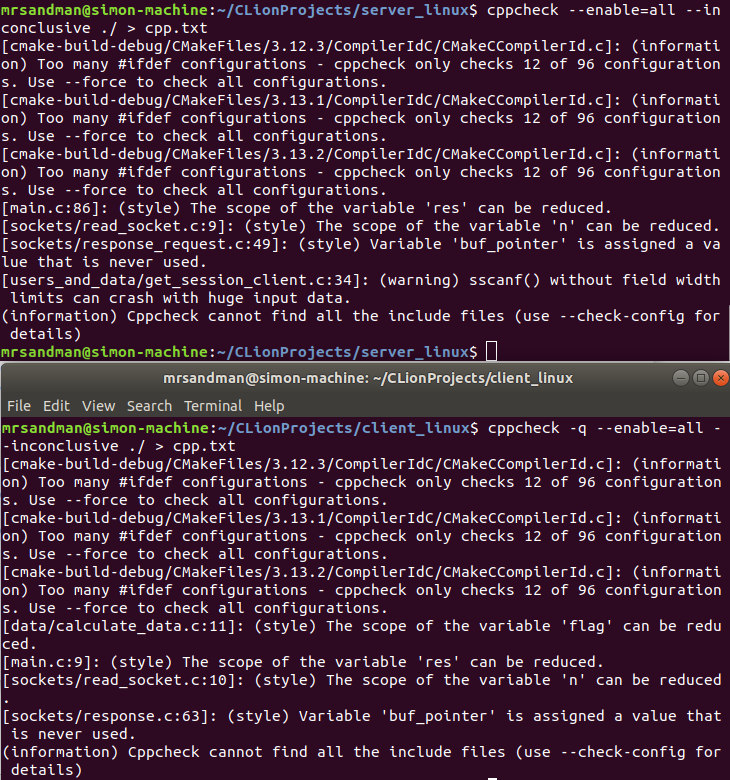
\includegraphics[scale=0.7]{cppcheck_tcp}
		\caption{Анализ клиента и сервера с помощью cppcheck} 
		\label{pic:cppcheck_tcp.png} % название для ссылок внутри кода
	\end{center}
\end{figure}

По полученным данным видно, что анализатор обратил внимание на использование переменных на слишком широком диапазоне, а также на возможность падения программы при большом объёме входных данных из-за использования sscanf без задания длины поля. Решением проблемы падения программы можно решить применением безопасной функции вместо sscanf.

	\item Динамические анализаторы кода
	
	Динамический анализ кода - это способ анализа программы непосредственно при ее выполнении. Процесс динамического анализа можно разбить на несколько этапов - подготовка исходных данных, проведение тестового запуска программы и сбор необходимых параметров, анализ полученных данных.
	
	С помощью динамического тестирования могут быть получены следующие метрики:
	
	\begin{itemize}
		\item Используемые ресурсы - время выполнения программы в целом или ее отдельных модулей, количество внешних запросов , количество используемой оперативной памяти и других ресурсов
		\item Цикломатическая сложность, степень покрытия кода тестами и другие метрики программы
		\item Программные ошибки - деление на ноль, разыменование нулевого указателя, утечки памяти, "состояние гонки"
		\item Наличие в программе уязвимостей.
	\end{itemize}

	Достоинства динамического анализа кода:
	
	\begin{itemize}
		\item В большинстве реализаций появление ложных срабатываний исключено, так как обнаружение ошибки происходит в момент ее возникновения в программе; таким образом, обнаруженная ошибка является не предсказанием, сделанным на основе анализа модели программы, а констатацией факта ее возникновения
		\item Зачастую не требуется исходный код; это позволяет протестировать программы с закрытым кодом
	\end{itemize}
	
	В качестве динамического анализатора была выбрана valgrind. Проверка была проведена для варианта индивидуального задания для протокола TCP.

\begin{figure}[H]
	\begin{center}
		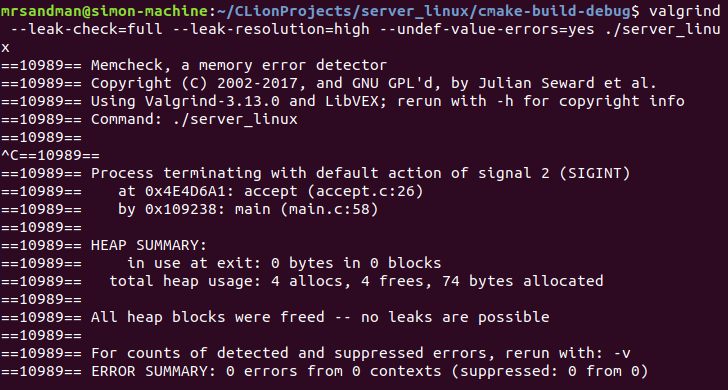
\includegraphics[scale=0.7]{valgrind_tcp_serv}
		\caption{Анализ сервера с помощью valgrind} 
		\label{pic:valgrind_tcp_serv.png} % название для ссылок внутри кода
	\end{center}
\end{figure}

\begin{figure}[H]
	\begin{center}
		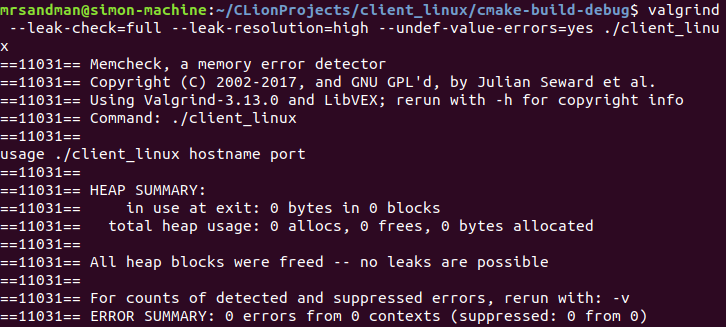
\includegraphics[scale=0.7]{valgrind_tcp_cli}
		\caption{Анализ клиента с помощью valgrind} 
		\label{pic:valgrind_tcp_cli} % название для ссылок внутри кода
	\end{center}
\end{figure}

По результатам анализа можно утверждать, что в ходе работы работы утечки памяти не возникают и отсутствуют неправильные использования многопоточности. Следовательно, дальнейших исправлений и улучшений не требуется.
\end{itemize}

\section{Выводы}
В ходе выполнения работы были разработаны 2 клиент-серверных приложения для обмена файлами: на TCP и UDP сокетах. Приложения работали согласно заданию, реализуя разработанный протокол, а также отлавливая ошибки при работе с сетью: ошибки при создании сокетов, соединении, приеме и передаче информации. 
 
TCP сервер должен был создавать отдельный сокет для каждого нового клиента, а также обмениваться сообщениями в отдельных потоках для каждого клиента. Также в TCP предусматривается возможность любого клиента по отдельности. UDP приложение не предусматривает общение с клиентами  в отдельных потоках, а также производит все через один сокет, но необходимо реализовать контроль пакетов: выявлять случаи потери или перемешивания пакетов.

При разработке протокола было принято решение о поддерживании сервером десяти команд для необходимых функций. Для удобства формирования и обработки команд все они были приведены к одному формату: команда + пробел + аргумент. Также для удобства было введено ограничение на длину команды в 1024 байт.

Также было выполнено дополнительное задание, подразумевающее запоминание состояния сервера при завершении работы. Для этого был создан текстовый файл, из которого при каждом запуске сервера выбираются все данные. Данные представлены в следующем формате: <текущий диапазон>;<диапазон для расчёта>;<список вычисленных простых чисел>. После каждого выполнения запроса CALC в файл записываются обновлённые данные.

При разработке приложения были написаны отдельные функции, вызываемые для каждой команды, для реализации исполнения этой команды как на стороне сервера, так и на стороне клиента. Это, а также общий формат для всех команд, позволило использовать и на стороне сервера и на стороне клиента одну функцию для обработки сообщения и определения введенной команды. Далее обмен производится в вызываемых при этом функциях. Однозначное соответствие функций клиента и сервера позволило облегчить как написание приложения, так и его отладку.

Для добавления контроля принятых пакетов на UDP приложении пришлось для каждого запроса и ответа на запрос запоминать его номер. В ходе обработки запроса ответу присваивается номер, который при передаче клиенту сравнивается с номером запроса. По несовпадающим номерам можно утверждать, что произошла потеря или перемешивание пакетов.

В ходе разработки приложения я столкнулся с проблемой постоянной отладки клиента и сервера, так как в языке C несовпадающие размеры буферов в связке recv/send могут привести к ошибке сегментации. Также возникла проблема с сохранением вычисленных данных в файл из-за очистки неопределённой части памяти. В связи с этим вместо работы с переменными типа FILE были использованы стандартные для ОС UNIX функции работы с файлами.
\end{document}
